\documentclass[11pt,a4paper]{article}
\usepackage[margin=2.3cm]{geometry}
\usepackage{amsmath,amssymb}
\usepackage{booktabs}
\usepackage{graphicx}
\usepackage{caption}
\usepackage{float}
\usepackage{xcolor}
\usepackage[hidelinks]{hyperref}
\usepackage{enumitem}
\usepackage{setspace}
\usepackage{tabularx}
\usepackage{lmodern}
\usepackage[round,authoryear]{natbib}
\usepackage[T1]{fontenc}
\captionsetup{font=small,labelfont=bf}
\setlist{itemsep=2pt,topsep=4pt}
\setstretch{1.04}
\newcommand{\unverified}{\textsuperscript{[U]}}

\title{\textbf{Funding Carry and Cross-Venue Arbitrage in Perpetual Futures:\\
A Pre-Registered Backtest of Hyperliquid against Binance and Bybit,\\ with a Review of the ATJ Research Approach}}
\author{Independent research}
\date{27 October 2026\\[4pt]\small Working paper. Paper research only: public data, no accounts, no orders.}

\begin{document}
\maketitle

\begin{abstract}
\noindent
This paper examines whether funding-rate differences in perpetual futures offer a tradeable edge to a small, base-fee-tier trader.
It first reviews the approach of ATJ Research, a retail educator who trades Hyperliquid perpetuals, including HIP-3 foreign-exchange and index markets such as \texttt{xyz:EUR}, \texttt{xyz:JPY} and \texttt{xyz:JP225}, against MetaTrader~5 (MT5) contracts for difference (CFDs). It then sets out perpetual-futures mechanics and the main arbitrage designs.
The empirical part is a pre-registered backtest on eight crypto majors (BTC, ETH, SOL, XRP, DOGE, SUI, LINK, AVAX) from 1 November 2024 to 26 October 2026, with the last three months held out of sample.
Costs are measured from live order books and charged on both legs.
A threshold-timed cross-venue funding-spread strategy earned $-0.20\%$ a year out of sample (Sharpe $-2.17$). All eight out-of-sample trades lost money, and costs were 267\% of gross funding.
A timed cash-and-carry (short Hyperliquid perpetual, long Binance spot) earned $+4.77\%$ in sample and $+3.13\%$ out of sample on allocated capital, which fails the pre-registered 4.5\% hurdle.
Always-on hedges did better on paper ($+5.36\%/+3.42\%$ perp/perp; $+5.86\%/+5.45\%$ perp/spot). However, a post-hoc stress test of the 10~October~2025 crash suggests that the perp/perp hedge at 2x leverage per leg would have lost roughly 19\% of capital in one day, and at 1x leverage the return falls below cash.
The Hyperliquid funding premium over centralised venues was positive in every quarter, but it narrowed from 19.3\% a year (2024Q4) to 2--9\% a year.
We conclude that the premium is real but, at retail costs and with realistic liquidation risk, it is roughly a cash-plus-zero-to-one-percent trade, not an arbitrage.
A second pre-registered study then tests the ATJ HL-against-CFD design on prop-firm demo MT5 bars (read-only proxy) versus trade.xyz HIP-3 markets. With next-bar fills, price-gap convergence earns $-7.8\%$ a year out of sample on total capital (almost no trades). Funding-versus-swap carry chosen in sample earns $-39\%$ out of sample. Both fail the pre-registered hurdle. Official trade.xyz fees are 0.009\%/0.003\% in growth mode and 0.090\%/0.030\% standard (gold is not growth-eligible); ATJ and an earlier note each quoted one of these.
\end{abstract}

\noindent\textbf{Keywords:} perpetual futures; funding rate; basis; cash-and-carry; Hyperliquid; HIP-3; limits to arbitrage; pre-registration.\\
\noindent\textbf{Notation:} \unverified{} marks a claim made by a content creator that has not been independently verified. ``HL'' = Hyperliquid; ``BIN'' = Binance USDT-M; ``BYB'' = Bybit linear; ``IS''/``OOS'' = in/out of sample. All returns are simple annualised returns on allocated capital unless stated otherwise.

{\small\tableofcontents}

%=====================================================================
\section{Literature review: ATJ Research and the academic literature}
\label{sec:lit}

\subsection{Sources and method}
The primary source for this section is an internal research note prepared before this paper (``\emph{Perps arbitrage: ATJ Research reality check}'', hereafter \emph{the note}; data pulled 26~October~2026, 17:13~GMT). It summarises ATJ Research's public material, a 30-day Hyperliquid data pull and a review of regulatory blockers.
We supplemented it with the public ATJ project page and strategy index \citep{atj_project,atj_strategies}, which we re-read on 27~October~2026, and with the auto-generated English captions of three ATJ YouTube videos (\citealp{atj_yt_bot,atj_yt_jpy,atj_yt_eur}; channel @ATJTraders618).
When the note was written, YouTube transcripts were rate-limited from our research machine (HTTP~429). \emph{That is no longer the case}: on 27~October~2026 the captions of all three videos were retrieved, and they are not redistributed with this repository. They are machine-generated and contain transcription errors. We quote them only for qualitative descriptions of the method and for the creator's own claims, which we mark as unverified.
The member area (\texttt{member.atjresearch.com}), which contains the code, screener, backtester and exact strategy files, sits behind a login and was not examined.

\subsection{What ATJ Research does}
\paragraph{Trade design.}
ATJ's project page describes a bot that ``identif[ies] arbitrage opportunities'' between Hyperliquid perpetuals on real-world assets (RWAs) and the corresponding MT5 CFDs: ``When the price difference is negative \ldots\ buy the HyperLiquid asset and sell the MT5 asset at the same time \ldots\ wait for price to return back to the mean'' \citep{atj_project}.
The creator uses IC~Markets as the MT5 broker and says he is migrating to a broker that supports USDC deposits ``to enable faster rebalancing and reducing USDC/USD conversion costs''.
The strategy index lists ``HyperLiquid / MT5 Arbitrage: \ldots\ Make money on the Spread and Funding Rates'' \citep{atj_strategies}.
The markets traded are HIP-3 builder-deployed perpetuals run by the deployer trade.xyz (prefix \texttt{xyz:}). The videos discuss \texttt{xyz:JPY} (USDJPY), \texttt{xyz:EUR} (EURUSD), \texttt{xyz:JP225} and an S\&P~500 market \citep{atj_yt_bot,atj_yt_jpy,atj_yt_eur}.

\paragraph{Signal: a grid centred on the funding--swap equilibrium.}
The two strategy guides describe a mean-reversion \emph{grid} on the cross-venue spread $s_t = P^{HL}_t - P^{MT5}_t$ \citep{atj_yt_jpy,atj_yt_eur}.
The grid centre is not zero. It is the spread at which Hyperliquid's hourly funding, annualised, equals the carry implied by the MT5 overnight swap: ``this is the price level where the funding rate on Hyperliquid and the swap values on MT5 should net zero in the ideal world'' \citep{atj_yt_jpy}.
For USDJPY the creator computes an implied annual rate of $-2.91\%$ from the midpoint of the IC~Markets long and short swaps (quoted as $+1.9\%$ and $-3.92\%$ a year). That gives a grid centre of $-0.08$ JPY with a grid step of 0.03--0.05 JPY.
For EURUSD the centre is $-0.0005$, derived from an assumed 1.5\% rate differential, with a step of 0.0005.
The creator stresses that MT5 swaps are marked up by the broker (for EURUSD: $-2.62\%$ a year long and $+0.44\%$ short), whereas Hyperliquid funding is peer-to-peer and symmetric.
The trade is therefore framed as ``both a spread arbitrage but also a funding rate arbitrage'' \citep{atj_yt_eur}.

\paragraph{Execution and stated risks.}
The guides model Hyperliquid fees of 0.006\% per side (one taker entry and one maker exit) for USDJPY, and quote trade.xyz fees of 0.009\% taker and 0.003\% maker in the EURUSD guide. An earlier note read trade.xyz \texttt{xyz} fees as 0.09\% taker and 0.03\% maker. Both figures are official: trade.xyz documents standard HIP-3 fees of 0.090\%/0.030\% and growth-mode fees of 0.0090\%/0.0030\%; gold is not growth-eligible \citep{tradexyz_fees}.
IC~Markets commission is quoted at USD~3.50 per lot per side \citep{atj_yt_eur}.
The creator acknowledges that one-minute snapshot backtests overstate profits because of spurious spikes, zero assumed slippage, adverse selection between the Hyperliquid fill and the MT5 hedge, and maker non-fills \citep{atj_yt_jpy}.
The project page lists execution, margin stop-out on one leg and pricing (oracle) risk \citep{atj_project}. The bot video calls one-leg liquidation ``the most important'' risk \citep{atj_yt_bot}.

\paragraph{Performance claims (all unverified).}
The videos report the following figures, which we have \emph{not} verified and which are not audited:
a live USD~100k account ``up 14\% over the past four months'', with USDJPY contributing about 6.7\% (the auto-caption also contains the phrase ``40\% and plus'', which contradicts it)\unverified{};
about 2\% (USD~19.37 on USDJPY) over the first two weeks of a new beta engine\unverified{} \citep{atj_yt_jpy};
a roughly USD~10k test account ``up 16\%'' or ``15.3\% since the beginning'' over about two months\unverified{};
and USD~2{,}400 (about 2.4\%) in the current month on the 100k account\unverified{} \citep{atj_yt_bot}.
The note could not read the public track-record dashboard, which is rendered with JavaScript.
The membership also sells an affiliate Hyperliquid sign-up and a prop-firm hedging simulator. This gives the creator a commercial interest in the strategy's appeal.

\subsection{What the note's data add}
The note pulled 720 hourly Hyperliquid prints (26~September to 26~October~2026).
Major crypto perpetuals traded a few basis points below the oracle on average, with a mean premium of $-3.37$~bp for BTC, $-2.67$~bp for ETH and $-3.72$~bp for SOL, and standard deviations of 1.3--2.3~bp.
\texttt{xyz:EUR} and \texttt{xyz:JPY} sat at steady offsets ($+2.99$ and $-3.35$~bp means, both with standard deviations of about 2.2~bp).
The note interprets these offsets as the interest-rate carry priced into a perpetual whose interest component trade.xyz sets to zero. They are a funding equilibrium, not a free spread.
Only the thin \texttt{xyz:JP225} market showed large gaps ($-53.5$ to $+24.7$~bp; standard deviation 8.27~bp), and its top five bid levels held only about USD~7{,}300 when sampled.
Table~\ref{tab:breakeven} reproduces the note's break-even comparison. On liquid markets the observed gaps are smaller than a realistic round-trip cost. The cleanest edge in the window was the funding carry on crypto majors, which motivates the backtest in Sections~\ref{sec:method}--\ref{sec:findings}.

\begin{table}[H]
\centering\small
\caption{Break-even comparison from the note (30-day window to 26 Oct 2026). The MT5 spreads are assumptions, not measurements.}
\label{tab:breakeven}
\begin{tabularx}{\textwidth}{Xccc}
\toprule
Trade & Round-trip cost & Observed signal & Verdict\\
\midrule
\texttt{xyz:EUR} vs EURUSD CFD, taker both legs & 21 bp & weekday $|$premium$|$ p95 5.5 bp, max 6.5 bp & below cost\\
Same, HL maker leg & 9 bp & same & below cost\\
\texttt{xyz:JP225} vs JP225 CFD, taker & 25 bp & p95 10.4 bp; 40--53 bp prints 28--29 Sep & rare, thin\\
BTC: HL short vs Binance long & 19 bp & 4.3\%/yr gap = 1.2 bp/day & 16 days to break even\\
BTC cash-and-carry on HL & 23 bp & 8.3\%/yr = 2.3 bp/day & 10 days to break even\\
\bottomrule
\end{tabularx}
\end{table}

\subsection{The academic literature}
\paragraph{Origins.}
\citet{shiller1993} proposed perpetual claims on cash-flow indices: a ``perpetual futures contract \ldots\ that would cash settle every day in terms of both the change in the futures price and the dividend or rent index''. The crypto perpetual swap, first listed by BitMEX in 2016, applied the idea with a funding payment in place of the dividend \citep{chitra2025adl}.

\paragraph{No-arbitrage pricing.}
\citet{ackerer2026} derive no-arbitrage prices for linear, inverse and quanto perpetuals. They show that the perpetual price equals the risk-neutral expectation of the spot sampled at a random time whose intensity reflects the funding specification. They also identify the interest terms that make the perpetual and spot prices coincide; for a linear contract this is a function of the two currencies' interest rates.
This is exactly the logic behind ATJ's grid centre. For an FX perpetual with no interest component, the no-arbitrage basis is the rate differential, not zero.
\citet{he2022} derive frictionless no-arbitrage prices and no-arbitrage \emph{bounds} under trading costs (``random-maturity arbitrage''). They document that crypto deviations from these bounds are larger than in traditional currency markets, comove across coins and diminish over time, and that an implied arbitrage strategy earns high Sharpe ratios.
That shrinking of deviations is consistent with the narrowing spread we report in Section~\ref{sec:regime}.

\paragraph{Carry and limits to arbitrage.}
\citet{schmeling2023} study the crypto futures basis (``crypto carry'') for BTC and ETH. They find that it averages above 10\% a year and sometimes exceeds 40\%, that it is driven by trend-chasing leveraged demand and scarce arbitrage capital constrained by margins and regulation, and that high carry predicts crashes.
\citet{makarov2020} document large, recurrent cross-exchange price deviations in bitcoin, especially across countries, and attribute them to frictions in moving arbitrage capital.
Both papers suggest that persistent crypto ``arbitrage'' returns are compensation for frictions and crash risk, not free money.
\citet{chitra2025adl} formalise auto-deleveraging (ADL) and analyse Hyperliquid's ADL on 10~October~2025, when about USD~2.1bn of positions were closed in roughly 12 minutes. This is the tail risk that a two-venue hedge carries (Section~\ref{sec:stress}).

\paragraph{Positioning of this paper.}
Relative to this literature our contribution is narrow and practical. We test a retail-implementable version of funding carry across one on-chain venue (Hyperliquid) and two centralised venues. We use costs measured from live order books, capital posted separately on each leg, and a pre-registered design with a held-out sample.

%=====================================================================
\section{Perpetual futures and arbitrage}
\label{sec:perps}

\subsection{Mechanics}
A perpetual future is a futures contract with no expiry. Because no terminal date forces convergence, an explicit periodic \emph{funding} payment between longs and shorts anchors the contract to a reference \emph{index} (oracle) built from spot prices.
When the perpetual trades above the index, longs pay shorts; when it trades below, shorts pay longs.
Funding is peer-to-peer: the venue does not trade against the user to push the price back.
This distinguishes it from a CFD broker's overnight \emph{swap}, which is a financing charge or credit set by the broker, usually with a mark-up, and booked at the daily rollover.

\subsection{Funding formulas and intervals}
Hyperliquid and the large centralised venues use the same template \citep{hl_funding,binance_funding}:
\begin{equation}
F = P + \operatorname{clamp}\!\left(I - P,\; -0.05\%,\; +0.05\%\right),
\label{eq:funding}
\end{equation}
where $F$ is the 8-hour funding rate, $P$ the time-averaged premium index and $I$ the interest component of 0.01\% per 8 hours.
Two consequences matter for carry trades:
\begin{itemize}
\item \textbf{The neutral rate.} When $|I-P|\le 0.05\%$ the clamp is inactive and $F=I$. So while the premium sits in roughly $[-0.04\%, +0.06\%]$ per 8 hours, shorts receive the interest component of 0.01\% per 8 hours, which is $0.01\% \times 3 \times 365 = 10.95\%$ a year in simple terms. Hyperliquid's documentation quotes this as ``11.6\% APR'' \citep{hl_funding}, which corresponds to hourly compounding of $0.00125\%$. We use the simple 10.95\% throughout.
\item \textbf{Intervals and caps.} Hyperliquid computes the 8-hour rate but \emph{pays one eighth of it every hour}. The premium is sampled every 5 seconds and averaged over the hour. Funding is capped at 4\% per hour, ``much less aggressive capping than CEX counterparts'' \citep{hl_funding}. Binance and Bybit settle every 8 hours for most symbols (some use 4h or 1h), with per-symbol caps \citep{binance_funding}.
\end{itemize}
On Hyperliquid the oracle is a liquidity-weighted median of centralised-exchange spot prices computed by each validator. The premium uses impact bid and ask prices for validator perpetuals, and for HIP-3 perpetuals it uses the mid of the impact prices over the oracle minus one. The payment is position size times \emph{oracle} price times rate \citep{hl_funding}.
On HIP-3 markets the deployer defines and pushes the oracle, sets a funding multiplier (0.5 on \texttt{xyz:EUR}, \texttt{xyz:JPY} and \texttt{xyz:JP225} as read by the note) and an interest rate (zero on \texttt{xyz:EUR}, \texttt{xyz:JPY} and \texttt{xyz:GBP}), and can halt and settle a market at mark \citep{hl_hip3}.
The \emph{mark} price, used for unrealised PnL and liquidation, differs from both the last trade and the oracle. Liquidation is triggered on mark, not on the last trade.

\subsection{Arbitrage designs}
\begin{enumerate}[label=(\roman*)]
\item \textbf{Cash-and-carry.} Buy spot and short the same notional of the perpetual, collecting funding while it is positive. The return is earned on the whole capital stack: spot fully paid plus perpetual margin.
\item \textbf{Cross-venue funding arbitrage (perp/perp).} Short the perpetual where funding is high and go long where it is low. The position is price-neutral and earns the funding \emph{difference}, with margin posted on both venues.
\item \textbf{Price-gap (basis) arbitrage against a reference.} ATJ's design: trade the perpetual's deviation from a liquid hedge (a CFD) and exit on mean reversion, collecting or paying funding versus swap in the meantime.
\end{enumerate}

\subsection{Risks}
\begin{itemize}
\item \textbf{Liquidation.} Margin is posted separately on each venue, so a large move liquidates the losing leg on one venue while the winning leg's profit sits on the other. With $L$x leverage per leg, a long leg is liquidated after a fall of roughly $1/L$ less the maintenance margin (about $-49\%$ at 2x in our calculation).
\item \textbf{Auto-deleveraging (ADL).} If liquidations cannot be filled, the venue force-closes profitable positions. This can close the \emph{hedge} leg and leave the other leg unhedged \citep{chitra2025adl}.
\item \textbf{Venue and counterparty risk.} Exchange failure, withdrawal halts, smart-contract and bridge risk (Hyperliquid collateral is bridged USDC), stablecoin risk and, on HIP-3, deployer discretion over the oracle, fees and settlement.
\item \textbf{Leg risk.} Sequential fills on two venues are exposed to price moves between fills and to partial fills.
\item \textbf{Funding-sign risk.} The funding spread can flip for weeks at a time.
\end{itemize}

%=====================================================================
\section{Idea and methodology}
\label{sec:method}

\subsection{Research question}
Is the funding premium paid on Hyperliquid over Binance and Bybit, noted in the note's 30-day pull, a persistent edge that survives realistic costs and capital requirements for a small trader on base-tier fees?
The design was written down and frozen in a pre-registration \emph{before} any backtest code was run \citep{prereg}. The deviations that followed are listed in Section~\ref{sec:deviations}.

\subsection{Data}
All data come from public, unauthenticated endpoints. No account, API key or wallet was used.
\begin{itemize}
\item \textbf{Funding:} Hyperliquid \texttt{fundingHistory} (hourly; 17{,}664 rows per coin from 20 October 2024), Binance \texttt{/fapi/v1/fundingRate} and Bybit \texttt{/v5/market/funding/history}.
\item \textbf{Prices:} 4-hour closes from Hyperliquid \texttt{candleSnapshot}, Binance USDT-M and spot klines, and Bybit linear klines. That is 4{,}417 4h bars and 2{,}209 8h funding prints per coin and venue.
\item \textbf{Costs:} order-book snapshots (Hyperliquid \texttt{l2Book}, Binance depth, Bybit orderbook) and Hyperliquid 1-minute candles.
\end{itemize}
All endpoints answered HTTP~200, so the pre-registered venue-substitution rule (OKX in place of Bybit, archive files in place of the Binance API) was not needed. No gaps were found inside the sample. The only incomplete bucket is the final one (26 October 2026, 00:00 UTC), which holds 7 of 8 Hyperliquid hourly prints \citep{carry_v1}.

\subsection{Universe and sample}
The universe is eight coins listed on all three venues: \textbf{BTC, ETH, SOL, XRP, DOGE, SUI, LINK, AVAX}. HYPE was excluded because its Binance USDT-M listing did not cover the full sample, and BNB because it is thin on Hyperliquid.
The full sample runs from \textbf{2024-11-01 to 2026-10-26} (UTC), limited by Hyperliquid's 4h candle history.
The in-sample period ends on 2026-07-26. The out-of-sample period, \textbf{2026-07-26 to 2026-10-26}, was held out and evaluated once, after the in-sample choices had been frozen.

\subsection{Time grid and accounting}
Decisions and accounting run on an 8-hour grid (00:00, 08:00 and 16:00 UTC).
Funding over $(t-8\text{h}, t]$ is the sum of the eight hourly Hyperliquid settlements, or of all Binance and Bybit settlements in that window.
Throughout, a positive rate means longs pay shorts.
The signal at $t$ uses only funding settled at or before $t$, and the position is held over $(t, t+8\text{h}]$.
Both legs are marked to market at every grid point (PnL = long-leg return minus short-leg return on notional $N$), so basis drift between the legs enters PnL directly.
Annualised return is the mean daily PnL divided by capital, times 365 (simple). Sharpe is the mean over the standard deviation of daily PnL times $\sqrt{365}$, with no risk-free rate deducted.

\subsection{Strategies}
\label{sec:strategies}
Equal notional $N$ per leg is used, delta-neutral at entry. The trailing signal window is $W=7$ days (21 periods) and was not tuned.
\begin{enumerate}[label=(\alph*)]
\item \textbf{Cross-venue funding spread.} 24 independent sleeves (8 coins $\times$ \{HL--BIN, HL--BYB, BIN--BYB\}). Let $s$ be the annualised 7-day mean of $f_A-f_B$. If flat and $s>\theta$, short $A$ and go long $B$; if $s<-\theta$, the reverse. Exit when the trailing spread in the held direction falls below $\theta/2$.
\item \textbf{Cash-and-carry.} Per coin: short the HL perpetual and buy Binance spot. Enter when the 7-day trailing HL funding (annualised) exceeds $\theta$; exit when it falls below $\theta/2$. Only the positive-funding direction is traded (spot is never shorted).
\item \textbf{Always-on baseline.} Per coin: short the HL perpetual and go long the Binance perpetual from the first to the last grid point. As a reference only, an always-on short HL perpetual with long Binance spot (``ref'') is also reported.
\end{enumerate}
The only tuned parameter, $\theta \in \{5, 10, 15, 20, 30\}\%$ a year, was chosen separately for (a) and (b) by in-sample portfolio Sharpe at base costs, then frozen. This selected \textbf{$\theta=15\%$ for (a)} and \textbf{$\theta=10\%$ for (b)} (Table~\ref{tab:grid}).

\subsection{Capital}
Margin is posted on each leg separately, with no cross-venue netting. The base case is 2x leverage per perpetual leg, so each perpetual leg needs $N/2$ of capital. Capital per sleeve is $N$ for (a) and (c), and $1.5N$ for (b) (spot fully funded plus $N/2$ of HL margin).
Capital is allocated to every sleeve for the whole sample and \emph{idle capital earns 0\%}. The portfolio holds equal capital per sleeve. Sensitivities at 1x and 3x leverage are reported.

\subsection{Cost model}
Costs were fixed before the run \citep{prereg}:
\begin{itemize}
\item \textbf{Fees} (base tier, taker on every fill, no discounts): HL perpetual 0.045\%, Binance USDT-M 0.050\%, Bybit linear 0.055\%, Binance spot 0.100\% \citep{hl_fees}.
\item \textbf{Slippage}: volume-weighted fill price versus mid for a USD~10k (base) or USD~100k (stress) market order per leg, averaged over buy and sell sides and over three snapshots taken 2 minutes apart (26 October 2026, 17:38--17:43 UTC). At USD~10k this is 0.01--0.3~bp for BTC and ETH and 0.4--2~bp for the other coins. The HL AVAX and SUI books (20 visible levels) cannot fill USD~100k, so under a rule fixed in advance they were assigned twice the worst other venue's figure.
\item \textbf{Leg risk}: the median absolute 1-minute return of each coin over the last 3 days of HL 1-minute candles (1.7~bp for BTC to 5.2~bp for SUI), charged once per entry and once per exit.
\end{itemize}
All-in round-trip costs at USD~10k are about 0.23\% of notional (BTC HL/BIN) to 0.36\% (SUI HL/BYB) for perp/perp, and 0.33\% (BTC) to 0.46\% (SUI) for HL perpetual against Binance spot \citep{carry_v1}.
Sensitivities: $0\times$, $0.5\times$, $1.5\times$ and $2\times$ the cost bundle; maker fees with no slippage; and USD~100k slippage.

\subsection{Pass/fail criteria (pre-registered)}
With a hurdle of a 4.5\% risk-free rate:
\begin{itemize}
\item \textbf{Real edge}: OOS net $>4.5\%$, OOS Sharpe $>1.5$ and OOS maximum drawdown $<5\%$; \emph{and} IS net $>4.5\%$; \emph{and} OOS net still $>0$ at 1.5x costs.
\item \textbf{Marginal}: OOS net $>0$, but at least one of the conditions above fails.
\item \textbf{No edge}: OOS net $\le 0$.
\end{itemize}
Strategies (a) and (b) are judged; (c) and ref are reference points.

\subsection{Deviations from the pre-registration}
\label{sec:deviations}
\begin{enumerate}
\item \textbf{Bug fixes after the first full run}, whose in-sample and out-of-sample summary had been seen. (i) The turnover counter always recorded zero. (ii) The cost of a decision taken at $t$ had been booked in period $(t-8\text{h}, t]$, so the first entry cost fell outside the in-sample window. Neither fix changed the selected $\theta$, and nothing was retuned. OOS numbers moved by less than 0.01 percentage points, and the in-sample return of (c) fell from 5.44\% to 5.36\% because its entry cost is now counted.
\item \textbf{Post-hoc stress analyses} (not used for pass/fail): a 1-minute mark-price check of the 10--11 October 2025 crash, and the maximum adverse move within trades on 8h closes. These can only make the results look worse.
\item The USD~100k HL slippage fill-in rule was fixed after the book snapshots were taken but before any backtest run.
\item The final 8h bucket has 7 of 8 HL prints. It was left as is; the effect is negligible.
\end{enumerate}

%=====================================================================
\section{Findings}
\label{sec:findings}

\subsection{Check of the note's funding claim}
Table~\ref{tab:fundcheck} recomputes 30-day and full-sample mean funding.
The note's headline holds: BTC funding over the 30 days to 26 October 2026 averaged \textbf{8.26\%} a year on Hyperliquid, against \textbf{3.79\%} on Binance and \textbf{3.83\%} on Bybit.
The note itself printed 3.95\% (Binance) and 3.97\% (Bybit) for BTC, and 8.01\% for ETH on HL, against 8.12\% in Table~\ref{tab:fundcheck}. These small differences reflect slightly different window boundaries and settlement aggregation. Where they differ we use the backtest files.
No venue funds above its neutral 10.95\%. Hyperliquid prints close to it, while Binance and Bybit print well below.

\begin{table}[H]
\centering\small
\caption{Mean annualised funding by venue. Source: \texttt{bt\_funding\_check.csv}. The 30-day window ends 26 Oct 2026; the full sample runs 1 Nov 2024 to 26 Oct 2026.}
\label{tab:fundcheck}
\begin{tabular}{lrrrrrr}
\toprule
 & \multicolumn{3}{c}{Last 30 days} & \multicolumn{3}{c}{Full sample}\\
\cmidrule(lr){2-4}\cmidrule(lr){5-7}
Coin & HL & BIN & BYB & HL & BIN & BYB\\
\midrule
BTC  & 8.26\% & 3.79\% & 3.83\% & 10.10\% & 5.09\% & 5.05\%\\
ETH  & 8.12\% & 3.85\% & 3.67\% & 9.60\% & 4.70\% & 5.25\%\\
SOL  & 6.81\% & 3.13\% & 2.35\% & 5.90\% & 1.05\% & 2.73\%\\
XRP  & 9.00\% & 3.21\% & 3.07\% & 7.98\% & 3.06\% & 4.43\%\\
DOGE & 9.66\% & 4.51\% & 2.91\% & 10.75\% & 4.88\% & 5.64\%\\
SUI  & 9.16\% & 4.62\% & 4.73\% & 8.12\% & 3.74\% & 6.26\%\\
LINK & 7.81\% & 3.62\% & 3.85\% & 13.21\% & 6.01\% & 5.72\%\\
AVAX & 4.87\% & 3.22\% & 3.32\% & 7.50\% & 1.68\% & 3.38\%\\
\bottomrule
\end{tabular}
\end{table}

\subsection{Portfolio results}
Table~\ref{tab:summary} gives the headline results and Figure~\ref{fig:cum} the cumulative net PnL.

\begin{table}[H]
\centering\small
\caption{Portfolio results (8 coins, equal capital per sleeve, base costs, 2x per leg). Net is annualised on allocated capital, including idle time. Source: \texttt{bt\_summary.csv}.}
\label{tab:summary}
\footnotesize\setlength{\tabcolsep}{3.2pt}
\begin{tabular}{llrrrrrrrr}
\toprule
Strategy & Period & Net & Sharpe & Max DD & In pos. & Net deployed & Turnover/yr & Trades & Hit\\
\midrule
(a) spread, $\theta$=15\% & IS  & 0.74\% & 2.26 & $-0.37\%$ & 11\% & 7.00\% & 11.4 & 118 & 54\%\\
                          & OOS & $\mathbf{-0.20\%}$ & $\mathbf{-2.17}$ & $-0.05\%$ & 2\% & $-8.82\%$ & 5.3 & 8 & \textbf{0\%}\\
(b) carry, $\theta$=10\%  & IS  & \textbf{4.77\%} & 7.76 & $-0.19\%$ & 54\% & 8.79\% & 11.2 & 56 & 70\%\\
                          & OOS & \textbf{3.13\%} & 7.75 & $-0.10\%$ & 68\% & 4.62\% & 17.2 & 15 & 87\%\\
(c) HL short / BIN perp   & IS  & \textbf{5.36\%} & 7.25 & $-0.43\%$ & 100\% & 5.36\% & 1.2 & -- & --\\
                          & OOS & \textbf{3.42\%} & 5.31 & $-0.14\%$ & 100\% & 3.43\% & 7.9 & 8$^\dagger$ & 100\%\\
ref: HL short / BIN spot  & IS  & \textbf{5.86\%} & 8.84 & $-0.29\%$ & 100\% & 5.86\% & 0.8 & -- & --\\
                          & OOS & \textbf{5.45\%} & 11.59 & $-0.12\%$ & 100\% & 5.47\% & 5.3 & 8$^\dagger$ & 100\%\\
\bottomrule
\end{tabular}

\smallskip\footnotesize $^\dagger$ The always-on trades are counted at the final exit (average hold 724 days), so the OOS cost line includes the one-off exit.
\end{table}

\begin{figure}[H]
\centering
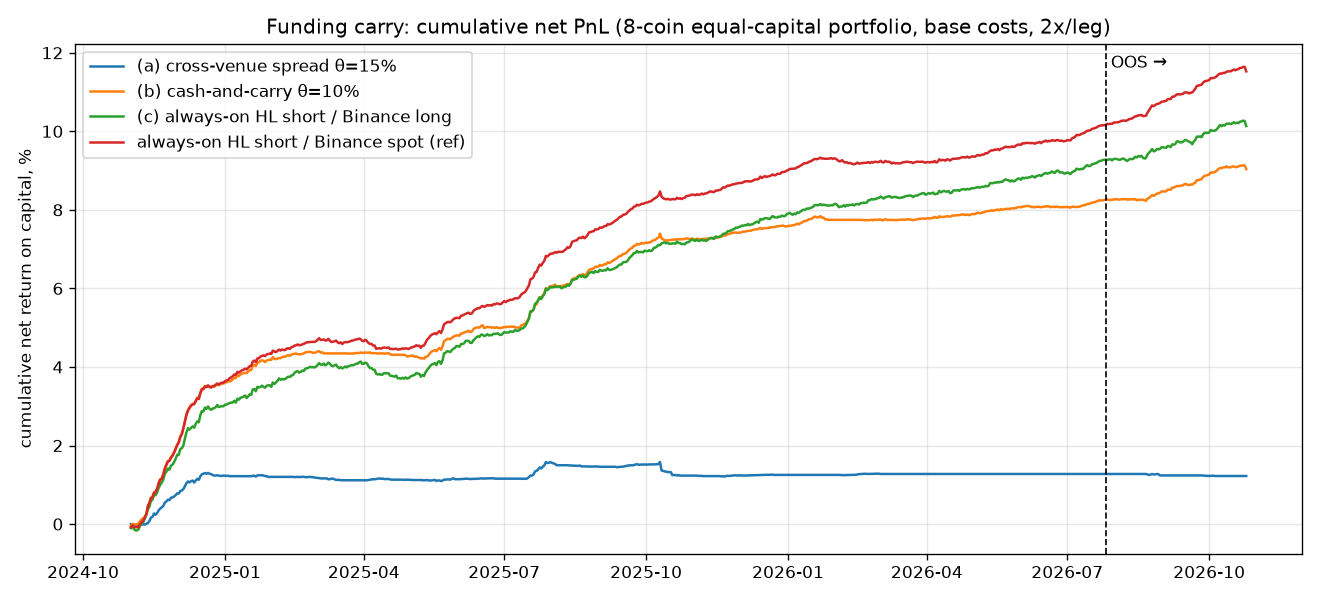
\includegraphics[width=\textwidth]{figures/cum_net_pnl.png}
\caption{Cumulative net return on capital for the four strategies (8-coin equal-capital portfolio, base costs, 2x per leg). The dashed line marks the start of the out-of-sample period (26 Jul 2026). Source: \texttt{backtest.py} output \texttt{cum\_net\_pnl.png}.}
\label{fig:cum}
\end{figure}

\paragraph{(a) Cross-venue spread: no edge.}
Out of sample, (a) lost 0.20\% a year with Sharpe $-2.17$, and all eight closed trades lost money (Table~\ref{tab:oos_a}).
In that quarter the 7-day spread rarely rose above the 15\% entry threshold. When it did, mainly in DOGE, SUI and LINK in late August and late September 2026, the trade's cost of 0.29--0.36\% of notional exceeded the funding collected over a hold of 2--8 days.
Even in sample, (a) earned only 0.74\% a year: it was deployed 11\% of the time, earning 7.00\% a year while deployed.
The Binance--Bybit sleeves lost money in sample in five of eight coins. There is no usable spread between the two centralised venues, and the only positive spread is between Hyperliquid and the centralised venues.

\begin{table}[H]
\centering\small
\caption{All eight out-of-sample trades of strategy (a). Funding, basis and cost are fractions of notional over the trade. Source: \texttt{bt\_trades\_a.csv}.}
\label{tab:oos_a}
\begin{tabular}{lllrrrr}
\toprule
Coin & Short/Long & Entry $\to$ exit (UTC) & Funding & Basis & Cost & Net\\
\midrule
DOGE & HL/BIN & 23 Aug 00:00 $\to$ 29 Aug 08:00 & 0.043\% & 0.044\% & 0.290\% & $-0.203\%$\\
DOGE & HL/BIN & 28 Sep 08:00 $\to$ 30 Sep 08:00 & 0.017\% & 0.036\% & 0.290\% & $-0.237\%$\\
DOGE & HL/BYB & 23 Aug 00:00 $\to$ 30 Aug 00:00 & 0.113\% & 0.133\% & 0.300\% & $-0.054\%$\\
DOGE & HL/BYB & 28 Sep 00:00 $\to$ 5 Oct 00:00 & 0.136\% & 0.064\% & 0.300\% & $-0.101\%$\\
SUI  & HL/BIN & 23 Aug 00:00 $\to$ 30 Aug 00:00 & 0.134\% & 0.072\% & 0.338\% & $-0.133\%$\\
SUI  & HL/BYB & 23 Aug 16:00 $\to$ 30 Aug 08:00 & 0.095\% & 0.013\% & 0.358\% & $-0.251\%$\\
LINK & HL/BIN & 22 Aug 16:00 $\to$ 30 Aug 00:00 & 0.163\% & $-0.016\%$ & 0.316\% & $-0.170\%$\\
LINK & HL/BYB & 22 Aug 08:00 $\to$ 30 Aug 00:00 & 0.245\% & 0.001\% & 0.330\% & $-0.085\%$\\
\bottomrule
\end{tabular}
\end{table}

\paragraph{(b) Cash-and-carry: marginal, fails the hurdle.}
Strategy (b) earned \textbf{+4.77\%} in sample and \textbf{+3.13\%} out of sample, with very low drawdowns (in sample $-0.19\%$, out of sample $-0.10\%$).
The out-of-sample return is below the pre-registered 4.5\% hurdle, so (b) is classified as \emph{marginal}. It stays positive at 2x costs out of sample ($+1.43\%$) and at 1.5x costs ($+2.28\%$), but it does not beat cash.

\paragraph{Always-on beats timing.}
Both always-on hedges beat both timed strategies. HL short against a Binance perpetual long earned \textbf{+5.36\%} in sample and \textbf{+3.42\%} out of sample; HL short against Binance spot earned \textbf{+5.86\%} and \textbf{+5.45\%}.
Timing the spread with thresholds destroyed value by adding turnover costs while cutting time in the market.
These high Sharpe ratios do not include liquidation risk, which the 8h grid hides (Section~\ref{sec:stress}).

\subsection{Cost decomposition}
Table~\ref{tab:costs} and Figure~\ref{fig:costs} decompose net returns.
For the timed strategies, fees, slippage and leg risk absorbed \textbf{55\%} of gross funding in (a) in sample and \textbf{267\%} out of sample, against 19\% and 37\% for (b).
Fees are by far the largest cost item. Slippage at USD~10k is small, and basis drift between the legs was small and slightly positive for the timed strategies.

\begin{table}[H]
\centering\small
\caption{Annualised decomposition, \% of capital. Source: \texttt{bt\_summary.csv} (columns \texttt{ann\_fund}, \texttt{ann\_basis}, \texttt{ann\_fee}, \texttt{ann\_slip}, \texttt{ann\_leg}).}
\label{tab:costs}
\begin{tabular}{llrrrrrrr}
\toprule
Strategy & Period & Gross fund. & Basis & Fees & Slippage & Leg risk & Net & Costs/gross\\
\midrule
(a) & IS  & 1.58 & 0.02 & $-0.56$ & $-0.10$ & $-0.20$ & 0.74 & 55\%\\
(a) & OOS & 0.16 & 0.06 & $-0.26$ & $-0.06$ & $-0.10$ & $-0.20$ & \textbf{267\%}\\
(b) & IS  & 5.73 & 0.14 & $-0.81$ & $-0.11$ & $-0.20$ & 4.77 & 19\%\\
(b) & OOS & 4.61 & 0.22 & $-1.25$ & $-0.16$ & $-0.29$ & 3.13 & 37\%\\
(c) & IS  & 5.55 & $-0.12$ & $-0.05$ & $-0.01$ & $-0.02$ & 5.36 & 2\%\\
(c) & OOS & 4.10 & $-0.11$ & $-0.38$ & $-0.06$ & $-0.13$ & 3.42 & 14\%\\
ref & IS  & 6.10 & $-0.16$ & $-0.06$ & $-0.01$ & $-0.01$ & 5.86 & 1\%\\
ref & OOS & 6.06 & $-0.09$ & $-0.38$ & $-0.05$ & $-0.09$ & 5.45 & 9\%\\
\bottomrule
\end{tabular}
\end{table}

\begin{figure}[H]
\centering
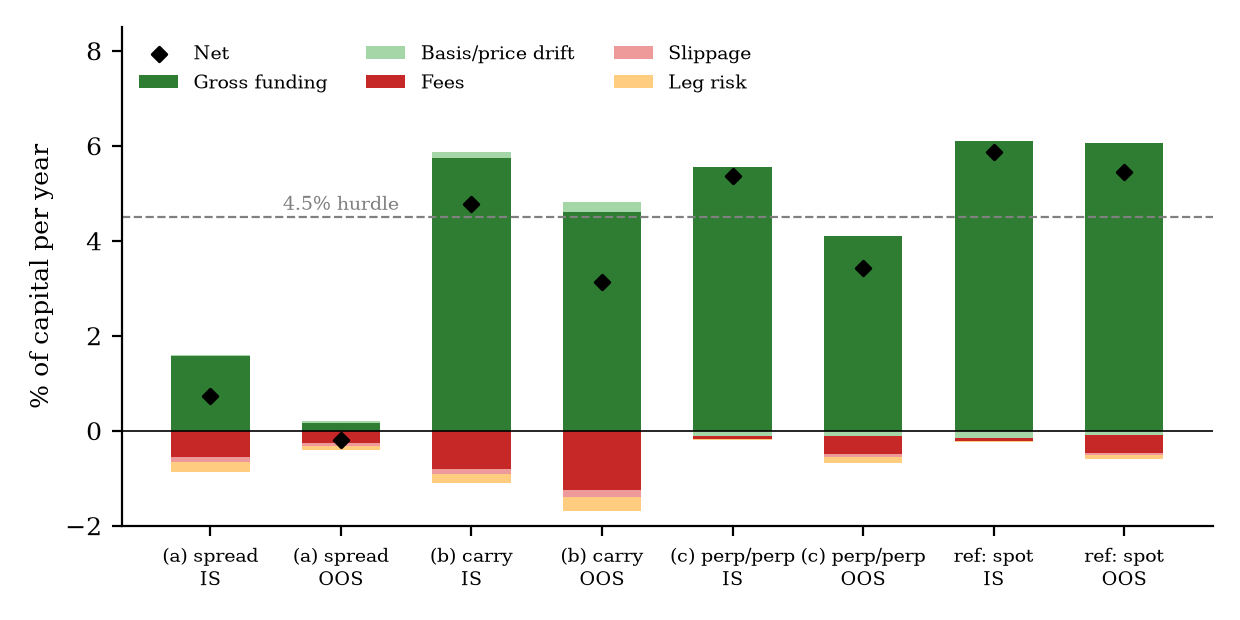
\includegraphics[width=0.92\textwidth]{figures/cost_breakdown.png}
\caption{Gross funding, basis drift and costs (stacked) with net return (diamonds) by strategy and period, in \% of capital per year. The dashed line is the 4.5\% pre-registered hurdle. Built by \texttt{make\_figures.py} from \texttt{bt\_summary.csv}.}
\label{fig:costs}
\end{figure}

\subsection{Threshold grid and sensitivity}
Table~\ref{tab:grid} reports the in-sample $\theta$ grid, and Table~\ref{tab:sens} the sensitivities with $\theta$ frozen.

\begin{table}[H]
\centering\small
\caption{In-sample $\theta$ grid (selection by IS Sharpe, then frozen). Source: \texttt{bt\_IS\_grid\_a.csv}, \texttt{bt\_IS\_grid\_b.csv}.}
\label{tab:grid}
\footnotesize\setlength{\tabcolsep}{4pt}
\begin{tabular}{rrrrrr@{\hspace{18pt}}rrrrr}
\toprule
\multicolumn{6}{c}{(a) cross-venue spread} & \multicolumn{5}{c}{(b) cash-and-carry}\\
\cmidrule(lr){1-6}\cmidrule(lr){7-11}
$\theta$ & Net & Sharpe & Max DD & In pos. & Trades & Net & Sharpe & Max DD & In pos. & Trades\\
\midrule
5\%  & 0.85\% & 1.87 & $-0.88\%$ & 47\% & 427 & 4.83\% & 7.53 & $-0.39\%$ & 71\% & 85\\
10\% & 0.83\% & 2.15 & $-0.54\%$ & 19\% & 206 & \textbf{4.77\%} & \textbf{7.76} & $-0.19\%$ & 54\% & 56\\
15\% & \textbf{0.74\%} & \textbf{2.26} & $-0.37\%$ & 11\% & 118 & 3.83\% & 6.83 & $-0.10\%$ & 32\% & 36\\
20\% & 0.61\% & 2.11 & $-0.34\%$ & 7\% & 74 & 2.80\% & 5.36 & $-0.09\%$ & 17\% & 30\\
30\% & 0.22\% & 1.11 & $-0.32\%$ & 3\% & 37 & 2.12\% & 4.51 & $-0.14\%$ & 10\% & 20\\
\bottomrule
\end{tabular}
\end{table}

\begin{table}[H]
\centering\small
\caption{Sensitivity of net annualised return on capital ($\theta$ frozen). Source: \texttt{bt\_sensitivity.csv}.}
\label{tab:sens}
\begin{tabular}{lrrrrrr}
\toprule
 & \multicolumn{2}{c}{(a) spread} & \multicolumn{2}{c}{(b) carry} & \multicolumn{2}{c}{(c) perp/perp}\\
\cmidrule(lr){2-3}\cmidrule(lr){4-5}\cmidrule(lr){6-7}
Variant & IS & OOS & IS & OOS & IS & OOS\\
\midrule
Cost $\times 0$   & 1.60\% & 0.21\% & 5.87\% & 4.82\% & 5.44\% & 3.99\%\\
Cost $\times 0.5$ & 1.17\% & 0.00\% & 5.32\% & 3.98\% & 5.40\% & 3.71\%\\
Cost $\times 1$ (base) & 0.74\% & $-0.20\%$ & 4.77\% & 3.13\% & 5.36\% & 3.42\%\\
Cost $\times 1.5$ & 0.30\% & $-0.41\%$ & 4.21\% & 2.28\% & 5.31\% & 3.13\%\\
Cost $\times 2$   & $-0.13\%$ & $-0.62\%$ & 3.66\% & 1.43\% & 5.27\% & 2.85\%\\
Maker fees, no slippage & 1.20\% & 0.02\% & 5.04\% & 3.54\% & 5.40\% & 3.72\%\\
USD 100k slippage & 0.36\% & $-0.35\%$ & 4.38\% & 2.53\% & 5.33\% & 3.21\%\\
1x leverage & 0.37\% & $-0.10\%$ & 3.57\% & 2.35\% & \textbf{2.68\%} & \textbf{1.71\%}\\
3x leverage & 1.11\% & $-0.31\%$ & 5.36\% & 3.52\% & 8.03\% & 5.13\%\\
\bottomrule
\end{tabular}
\end{table}

\noindent Even with zero costs, (a) earns only 0.21\% a year out of sample, so the entry rule, not just the costs, is the problem.
Maker-only execution lifts (b) out of sample to 3.54\%, still below the hurdle.
Leverage only rescales capital and leaves Sharpe unchanged. 3x per leg lifts (c) to 8.03\% in sample and 5.13\% out of sample, but it worsens the liquidation exposure discussed below.

\subsection{Funding regime: does the Hyperliquid premium persist?}
\label{sec:regime}
Table~\ref{tab:quarter} and Figure~\ref{fig:quarter} give the 8-coin mean funding by quarter. Figure~\ref{fig:spread} shows the 30-day rolling spreads per coin.

\begin{table}[H]
\centering\small
\caption{Mean annualised funding across the 8 coins by calendar quarter (2024Q4 starts 1 Nov; 2026Q4 ends 26 Oct). Computed from \texttt{bt\_funding\_by\_quarter.csv}.}
\label{tab:quarter}
\begin{tabular}{lrrrrr}
\toprule
Quarter & HL & BIN & BYB & HL$-$BIN & HL$-$BYB\\
\midrule
2024Q4 & 34.05\% & 14.78\% & 20.61\% & \textbf{19.28\%} & 13.44\%\\
2025Q1 & 6.59\% & 2.16\% & 4.64\% & 4.42\% & 1.94\%\\
2025Q2 & 6.23\% & 2.88\% & 3.58\% & 3.35\% & 2.64\%\\
2025Q3 & 15.45\% & 6.89\% & 7.86\% & 8.56\% & 7.59\%\\
2025Q4 & 5.18\% & 1.48\% & 0.29\% & 3.69\% & 4.89\%\\
2026Q1 & 1.38\% & $-0.68\%$ & 1.00\% & 2.06\% & 0.37\%\\
2026Q2 & 3.45\% & 1.17\% & 1.92\% & 2.27\% & 1.52\%\\
2026Q3 & 9.39\% & 5.14\% & 4.20\% & 4.25\% & 5.19\%\\
2026Q4 & 7.44\% & 3.45\% & 3.12\% & 3.98\% & 4.32\%\\
\bottomrule
\end{tabular}
\end{table}

\begin{figure}[H]
\centering
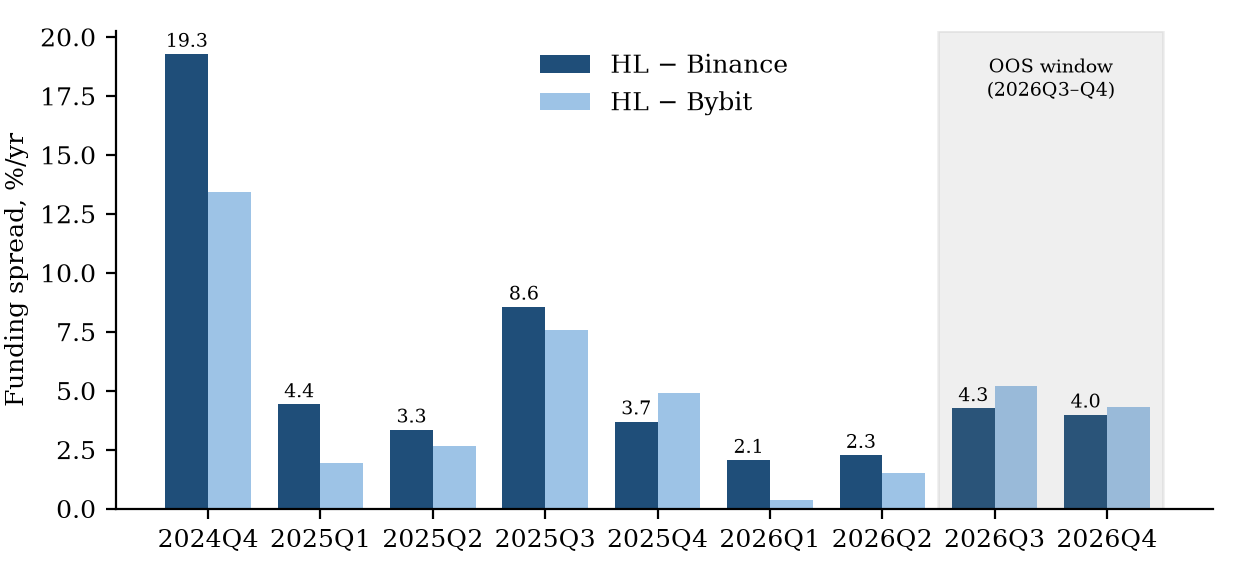
\includegraphics[width=0.9\textwidth]{figures/quarterly_spread.png}
\caption{Quarterly 8-coin mean HL$-$Binance and HL$-$Bybit funding spread, \%/yr. The shaded area covers the quarters that overlap the out-of-sample window. Built by \texttt{make\_figures.py} from \texttt{bt\_funding\_by\_quarter.csv}.}
\label{fig:quarter}
\end{figure}

\noindent The HL$-$centralised-venue spread was positive in every quarter on the 8-coin average.
It fell from \textbf{19.3\%} a year in 2024Q4, a bullish, high-funding regime, to between 2.1\% and 8.6\% a year against Binance from 2025Q1 onwards. The weakest stretch was 2026Q1--Q2 (about 2.1--2.3\% against Binance and 0.4--1.5\% against Bybit), and SOL and XRP were negative against Binance in 2026Q1.
Spread levels track the funding regime: high-funding bull markets widen the spread and choppy markets compress it.
The rolling series (Figure~\ref{fig:spread}) go negative for weeks at a time, for example in April 2025 and February--May 2026. These are the periods in which the always-on hedges bleed.
The narrowing is consistent with the finding of \citet{he2022} that deviations diminish over time.

\begin{figure}[H]
\centering
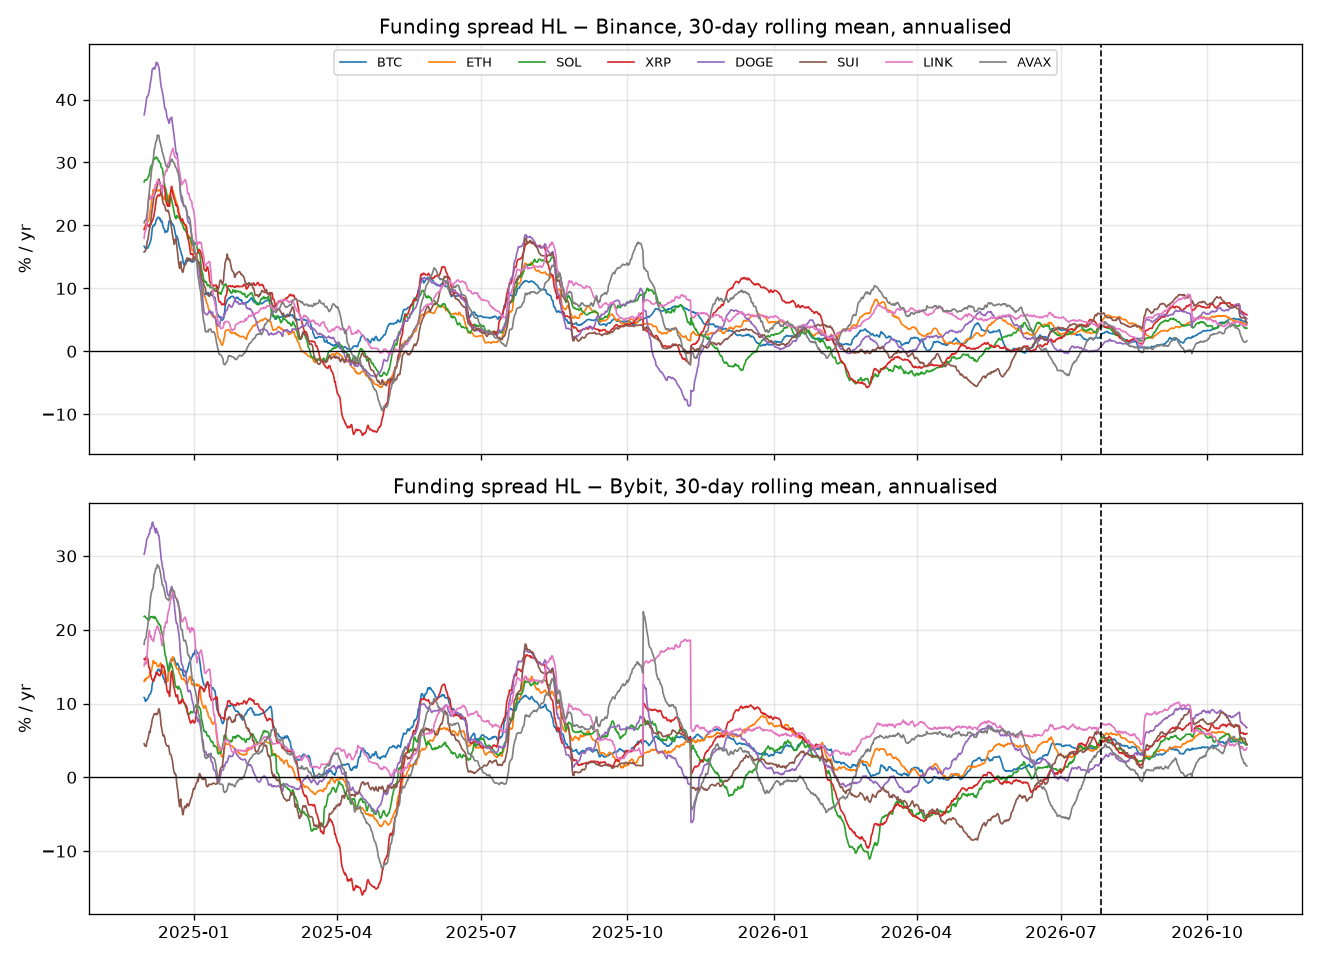
\includegraphics[width=\textwidth]{figures/funding_spread.png}
\caption{30-day rolling HL$-$Binance and HL$-$Bybit funding spread per coin, annualised; the vertical line marks the OOS start. Source: \texttt{backtest.py} output \texttt{funding\_spread.png}.}
\label{fig:spread}
\end{figure}

\subsection{Tail risk: the 10 October 2025 crash}
\label{sec:stress}
The 8h-close accounting hides intrabar wicks. The worst 7-day episodes on 8h closes were small, for example $-0.66\%$ of sleeve capital for XRP in (c) in the week to 7 April 2025 \citep{carry_v1}.
Table~\ref{tab:wick} reports the worst 1-minute \emph{mark}-price lows, the prices used for liquidation, between 12:00 UTC on 10 October 2025 and 12:00 UTC the next day.

\begin{table}[H]
\centering\small
\caption{Worst move against the 12:00 UTC open, 10--11 Oct 2025 (24h window). Source: \texttt{oct10\_2025\_wick\_check.txt}.}
\label{tab:wick}
\begin{tabular}{lrrrr}
\toprule
Coin & Binance mark 1m low & Binance mark 24h later & Bybit mark 1m low & Liquidated at 2x?\\
\midrule
BTC  & $-16.2\%$ & $-7.6\%$  & $-12.2\%$ & no\\
ETH  & $-21.1\%$ & $-11.6\%$ & $-15.8\%$ & no\\
SOL  & $-34.9\%$ & $-17.0\%$ & $-26.2\%$ & no (yes at 3x)\\
XRP  & $-57.7\%$ & $-12.1\%$ & $-55.2\%$ & \textbf{yes}\\
DOGE & $-64.6\%$ & $-22.7\%$ & $-61.5\%$ & \textbf{yes}\\
SUI  & $-83.3\%$ & $-21.7\%$ & $-82.5\%$ & \textbf{yes}\\
LINK & $-63.8\%$ & $-19.5\%$ & $-62.8\%$ & \textbf{yes}\\
AVAX & $-69.9\%$ & $-19.8\%$ & $-68.6\%$ & \textbf{yes}\\
\bottomrule
\end{tabular}
\end{table}

\noindent At 2x per leg a long perpetual is liquidated at roughly $-49\%$, so the always-on HL-short/Binance-long hedge would have lost its long leg in five of eight coins.
Our rough estimate for each affected sleeve: the long leg's margin is lost ($-50\%$ of sleeve capital) and is partly offset by the short leg's gain measured at the price 24 hours later (Table~\ref{tab:wick}). That gives $-37.9\%$ (XRP), $-27.3\%$ (DOGE), $-28.3\%$ (SUI), $-30.5\%$ (LINK) and $-30.2\%$ (AVAX), and summed over eight equal sleeves about \textbf{$-19\%$ of portfolio capital in one day} ($-19.3\%$ by our arithmetic). That is roughly 3.5 years of carry.
The estimate assumes no collateral top-up during a wick lasting minutes and ignores liquidation fees and ADL. It is a post-hoc, order-of-magnitude figure, not a backtest result.
At 3x per leg SOL is also liquidated. At 1x no leg is liquidated (SUI's $-83\%$ low is above the threshold of about $-99\%$), but returns halve to \textbf{+2.68\%} in sample and \textbf{+1.71\%} out of sample, which is below cash.
Strategy (a) had two AVAX sleeves open that day (HL short against Binance and against Bybit), so it was exposed in the same way.

The cash-and-carry leg cannot be liquidated on the spot side, but its HL short is exposed to rallies. On 8h closes, the HL price rose by up to +550\% (XRP), +189\% (DOGE) and +166\% (LINK) within single (b) trades opened on 1 November 2024 (\texttt{liquidation\_stress.txt}). In the always-on series, the maximum HL run-up from 1 November 2024 was +608\% for XRP.
Without regular collateral transfers from Binance to Hyperliquid, those short legs would have been liquidated. The backtest assumes costless 8h resizing and costless collateral rebalancing.
Finally, Hyperliquid ran cross-margin ADL on 10 October 2025, closing about USD~2.1bn of positions in roughly 12 minutes \citep{chitra2025adl}. ADL can force-close the profitable hedge leg and leave the other leg unhedged.

\subsection{Verdict against the pre-registered criteria}
\begin{table}[H]
\centering\small
\caption{Verdict against the criteria in Section~\ref{sec:method}.}
\label{tab:verdict}
\begin{tabular}{lccccccl}
\toprule
 & OOS net & OOS Sharpe & OOS DD & IS net & OOS at 1.5x & & \\
 & $>$4.5\% & $>$1.5 & $<$5\% & $>$4.5\% & $>$0 & & Verdict\\
\midrule
(a) & $-0.20\%$ & $-2.17$ & $-0.05\%$ & 0.74\% & $-0.41\%$ & & \textbf{No edge}\\
(b) & 3.13\% & 7.75 & $-0.10\%$ & 4.77\% & 2.28\% & & \textbf{Marginal} (fails OOS hurdle)\\
\bottomrule
\end{tabular}
\end{table}

%=====================================================================
\section{HIP-3 versus MT5 CFD leg (prop-firm demo feed proxy)}
\label{sec:cfd}

This section reports a second pre-registered study of ATJ's HL-against-CFD design
(\texttt{perps-arb/preregistration\_cfd.md}, written 27~October~2026 07:48~UTC before any strategy PnL).
It uses a \emph{read-only} copy of prop-firm demo MT5 broker bars and a single swap snapshot, plus public Hyperliquid
\texttt{info} endpoints for trade.xyz (\texttt{xyz:}) HIP-3 markets. No accounts, keys, wallets or orders were used.

\paragraph{Hard caveat.}
prop-firm demo feed is a prop-firm demo feed, not the retail broker ATJ uses.
The prop firm's general terms ban exploiting price feeds, latency or arbitrage.
Results are therefore a proxy for gap and cost structure only, not a tradable setup.

\subsection{Universe, data and costs}
Seven mapped pairs: \texttt{xyz:EUR}/\texttt{EURUSD}, \texttt{xyz:GBP}/\texttt{GBPUSD},
\texttt{xyz:JPY}/\texttt{USDJPY}, \texttt{xyz:GOLD}/\texttt{XAUUSD},
\texttt{xyz:JP225}/\texttt{JP225.cash}, \texttt{xyz:SP500}/\texttt{US500.cash},
\texttt{xyz:XYZ100}/\texttt{US100.cash} (the demo feed lists US100, not NAS100).
There is no HL Dow market; \texttt{US30.cash} is excluded from trading tests.
HL \texttt{candleSnapshot} returns at most about 5000 candles and does not page earlier, so
1h history begins around 1~April~2026 (GBP from 18~May; JP225 from 9~April) and 1m history only from about 23~October~2026.
MT5 parquets end 7~October~2026, so there is \textbf{no M1 overlap}; strategies (A) and (C) use aligned H1 bars
(deviation logged in the pre-registration).
The frozen IS/OOS split (\texttt{results/cfd/sample\_split.json}) is 1~April--30~August~2026 IS and
30~August--7~October~2026 OOS (189 calendar days total).

MT5 bars are bid OHLC; mid $= \mathrm{bid} + \tfrac12\times\mathrm{spread}\times\mathrm{point}$
using inventory/live spreads (not the cost table known to double-count spread).
Commission is \$5 per lot round trip for FX/metals and zero for indices.
Swaps for all eight symbols come from a 27~October~2026 07:43~UTC snapshot and are held constant historically;
triple swap is Wednesday for FX/gold and Friday for indices.
HL fees follow the official trade.xyz schedule: growth-mode 0.0090\%/0.0030\% where meta shows
\texttt{growthMode}, and standard 0.090\%/0.030\% for gold.
Headline pass/fail uses this docs-correct schedule with taker fees on both sides.
Capital is posted on both legs (prop-firm-style 1:100 CFD margin plus HL max-leverage margin) and returns are on total capital.

\subsection{Strategies and pass/fail}
(A) Price-gap convergence on H1: enter when $|$HL mid $-$ MT5 mid$|$ exceeds a threshold net of round-trip costs
plus a leg-risk penalty; exit on half-threshold or timeout; \textbf{next-bar fills} (no same-bar look-ahead).
(B) Always-on carry: hold HL one way against the MT5 CFD, collecting funding minus swap; direction chosen on IS only.
(C) Passive measurement of the gap distribution and half-life.
Hurdle: OOS net annualised on capital $>4.5\%$, Sharpe $>1.5$, max DD $<10\%$, and still positive at $1.5\times$ costs.

\subsection{Findings}
Passive H1 gaps are small: typical mean absolute offsets of about 0--3~bp and standard deviations of 3--8~bp
(JP225 about 16~bp), with AR(1) half-lives of roughly 0.6--2.7 hours
(Figure~\ref{fig:cfd_gap_hist}).
Round-trip docs-correct costs are about 2--3~bp on growth-mode pairs and about 19~bp on gold (standard fees).
Same-bar fills produced a spurious GBPUSD gap ``edge''; under next-bar execution that collapsed.

\begin{figure}[H]
\centering
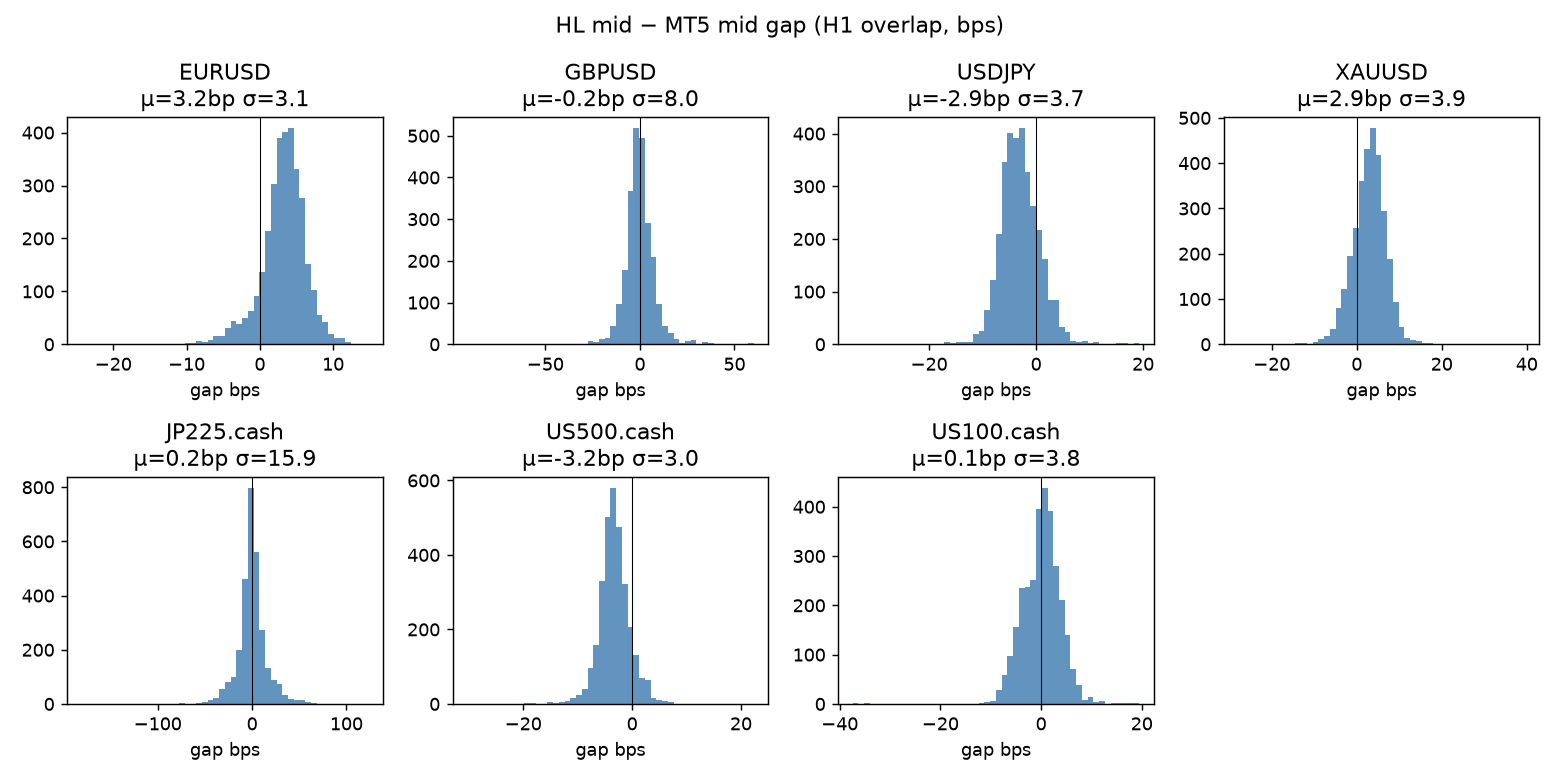
\includegraphics[width=0.95\textwidth]{figures/gap_histograms.png}
\caption{Distribution of the H1 gap (HL mid minus MT5 mid, basis points) over the overlapping sample to 7~October~2026.}
\label{fig:cfd_gap_hist}
\end{figure}

\begin{table}[H]
\centering
\caption{HIP-3 vs MT5 CFD portfolio results (docs-correct fees, \$10k notional per leg, return on total capital).}
\label{tab:cfd_port}
\small
\begin{tabular}{@{}llrrr@{}}
\toprule
Strategy & Period & Net (\$) & Ann.\ on capital & Trades \\
\midrule
(A) gap, $\theta=80$~bp, $T=30$m & IS & $-51$ & $-4.5\%$ & 1 \\
(A) gap & OOS & $-22$ & $-7.8\%$ & 1 \\
(B) carry, IS-chosen direction & IS & $+94$ & $+8.9\%$ & 7 pairs \\
(B) carry & OOS & $-111$ & $-39.0\%$ & 7 pairs \\
\bottomrule
\end{tabular}
\end{table}

\begin{figure}[H]
\centering
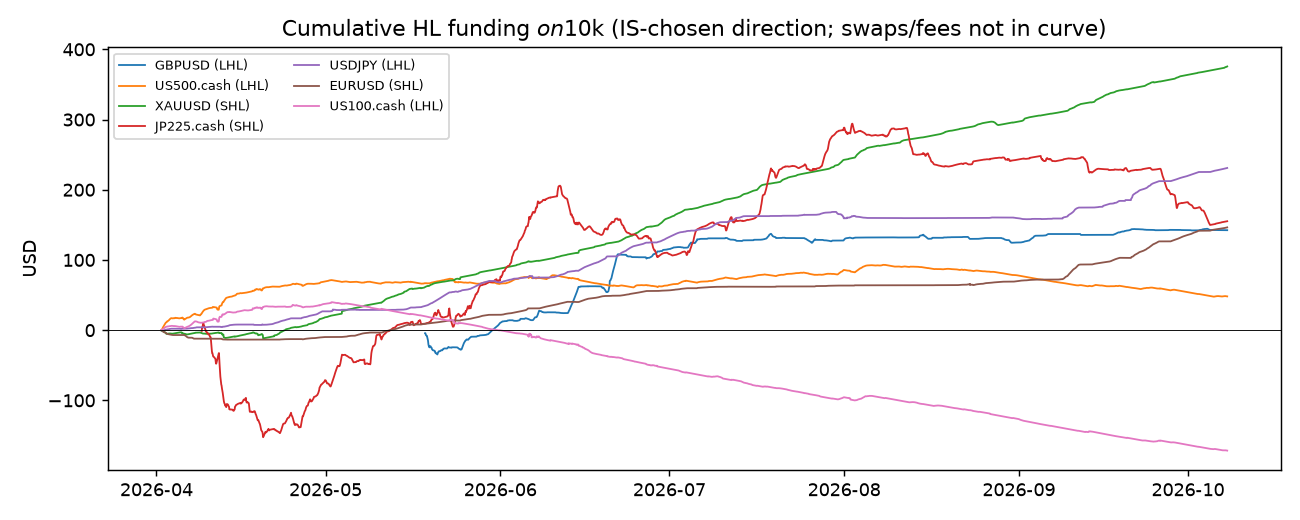
\includegraphics[width=0.95\textwidth]{figures/carry_cum_funding.png}
\caption{Cumulative HL funding dollars on \$10k notional in the IS-chosen carry direction (swaps and fees not in the curve).}
\label{fig:cfd_carry}
\end{figure}

\noindent\textbf{Verdict:} (A) \textbf{no edge}; (B) \textbf{no edge}.
A few pairs (notably GBPUSD and XAUUSD carry on the full window) look positive in isolation, but
JP225 and US100 losses dominate the equal-capital book out of sample.
Full tables and code live under \texttt{perps-arb/results/cfd/} and \texttt{perps-arb/pipeline/cfd/}.

%=====================================================================
\section{Discussion and limitations}
\label{sec:discussion}

\subsection{Interpretation}
The Hyperliquid funding premium is real and has lasted for two years. Hyperliquid prints near its 10.95\% neutral rate, while Binance and Bybit print well below theirs.
A passive harvest earns about 5\% a year on capital at 2x per leg, but carries a tail of roughly $-19\%$ in a single day. At 1x, which survives the October 2025 crash, it earns about 2--3\% a year. That is cash plus 0--1\% at best, before venue and counterparty risk, and less than cash at 1x.
This matches the limits-to-arbitrage reading of \citet{schmeling2023} and \citet{makarov2020}: the carry pays for margin constraints, crash risk and venue frictions.
Threshold timing on a 7-day window \emph{subtracted} value, because the spread rarely moved enough to cover a 0.23--0.46\% round trip.

For ATJ's design the implication is indirect but consistent. The FX perpetual offsets on \texttt{xyz:EUR} and \texttt{xyz:JPY} are mostly carry, as \citet{ackerer2026} would predict for a contract with no interest component, and the remaining noise in the note's hourly data (p95 about 5.5~bp) is below the estimated 9--21~bp round trip.
Profits, if any, would have to come from intrahour dislocations, maker rebates or thin markets such as \texttt{xyz:JP225}. All three are hard to verify and limited in capacity.

\subsection{Limitations}
\begin{itemize}
\item \textbf{8h bars miss intrabar liquidation.} PnL is marked on 4h closes sampled every 8h. Section~\ref{sec:stress} shows that this hides the most important risk. The liquidation estimate is rough and post-hoc.
\item \textbf{Collateral transfers are not modelled.} Rebalancing margin between venues (withdrawal fees, bridge time, USDC/USDT conversion) is assumed costless and instantaneous. So is the 8h resizing to constant notional.
\item \textbf{Idle capital earns 0\%} in the headline. Crediting T-bill or stablecoin yield on idle cash would raise (a) and (b) but is not an edge. The relevant comparison is carry against cash.
\item \textbf{Single cost snapshot.} Slippage and leg risk come from one 5-minute window on a weekday evening. Spreads widen in volatile markets, exactly when an exit may be needed.
\item \textbf{One spot venue} (Binance) and base-tier fees. Funding-rate caps, tiered margin and the actual liquidation engines are not modelled.
\item \textbf{Short OOS sample.} The OOS window is one quarter (about 270 8h periods), so OOS Sharpe ratios are noisy.
\item \textbf{CFD leg is a prop-firm demo feed proxy.} Section~\ref{sec:cfd} uses prop-firm demo feed bars and a single swap snapshot, not ATJ's retail broker. Live ticks (10--24~Oct~2026) do not overlap the parquet window (ends 7~Oct), so bid-versus-mid identity inside the sample cannot be confirmed bar-by-bar. Historical swaps are assumed constant. HL 1m history does not overlap MT5, so gap tests use H1. ATJ's live claims remain unverified on his venue.
\end{itemize}

\subsection{Regulatory and practical blockers (for the reader to verify)}
The following items are stated neutrally. They are drawn from the note and re-checked where noted. They are not legal advice, and the reader should verify each before acting.
\begin{itemize}
\item \textbf{trade.xyz terms.} Section~2.2(a) of the trade.xyz Terms of Use (last updated 6 September 2026) lists persons who reside in, are located in or are subject to the laws of ``the United States of America, Canada, the United Kingdom'' as Restricted Persons, and Section~2.3 prohibits circumvention by VPN \citep{tradexyz_terms}; re-read 27 October 2026. trade.xyz deploys the \texttt{xyz:} markets that ATJ trades.
\item \textbf{FCA Warning List.} The FCA lists Hyperliquid (first published 21 May 2026, updated 7 June 2026) as a firm that ``is not authorised by us and may be targeting people in the UK''. Users would have no access to the Financial Ombudsman Service or the FSCS \citep{fca_hl}; re-read 27 October 2026.
\item \textbf{FCA retail crypto-derivatives ban.} COBS~22.6 bars firms from selling crypto derivatives to UK retail clients \citep{fca_cobs226}. It binds firms, not individuals.
\item \textbf{CFD broker terms on arbitrage.} According to the note, IC~Markets' Order Execution Policy reserves the right to cancel orders, close accounts and recover losses for arbitrage including ``latency arbitrage'' and ``swap arbitrage'' \citep{icm_oep}. Other brokers' terms differ and should be read in full.
\end{itemize}

%=====================================================================
\section{Conclusion and future work}
\label{sec:conclusion}
Funding-rate arbitrage between Hyperliquid and the large centralised venues is, on this evidence, \emph{not} an arbitrage for a small trader on base-tier fees. The threshold-timed spread strategy failed out of sample (no edge), the timed cash-and-carry failed the hurdle (marginal), and the always-on hedges that look best on 8h data carry a crash tail that, at 2x per leg, would have cost about three and a half years of carry in a single day. The separate HIP-3 versus MT5 CFD proxy likewise shows no edge for price-gap convergence or funding-versus-swap carry once next-bar fills and docs-correct fees are applied.
The premium itself is durable but has narrowed sharply since late 2024.
Any further work requires a new pre-registration. In priority order:
\begin{enumerate}
\item \textbf{Always-on carry at 1--1.5x} with explicit collateral rebalancing rules and costs, and liquidation modelled on 1-minute mark prices, including 10 October 2025 and ADL.
\item \textbf{Slower spread signals} (30--60 day) for entry and exit in place of a 7-day threshold, with maker-only (post-only, 0.015\%) execution on Hyperliquid.
\item \textbf{Live collector validation}: run the existing one-shot collector hourly for several weeks to test whether snapshot costs hold and how predicted funding compares with realised funding.
\item \textbf{Universe extension}: HYPE and other Hyperliquid-native names, where the premium may be larger but history is shorter, and OKX as a fourth venue.
\item \textbf{Comparison with stablecoin and cash yield}: set the carry next to the yield actually available on idle USDC/USDT (on-venue) or T-bills, since the real decision is carry against cash.
\end{enumerate}
The prop-firm demo feed proxy of ATJ's HL-against-CFD design (Section~\ref{sec:cfd}) also shows no edge under pre-registered costs and next-bar fills; any follow-up would need a new pre-registration, overlapping tick-level data from a retail CFD feed the researcher may lawfully use, and resolution of the access issues in Section~\ref{sec:discussion}.

\section*{Data and code availability}
\sloppy
Pre-registrations: \texttt{perps-arb/preregistration.md} (crypto) and \texttt{perps-arb/preregistration\_cfd.md} (HIP-3/CFD). Pipelines: \texttt{perps-arb/pipeline/} and \texttt{perps-arb/pipeline/cfd/}. Results: \texttt{perps-arb/results/} and \texttt{perps-arb/results/cfd/}. Extra figures: \texttt{perps-arb/paper/make\_figures.py}. Every number in this paper is taken from these files, from the note, or from the cited official docs.

%=====================================================================
\begin{thebibliography}{99}
\setlength{\itemsep}{2pt}\small

\bibitem[Ackerer et al.(2026)]{ackerer2026}
Ackerer, D., Hugonnier, J., and Jermann, U. (2026). Perpetual futures pricing. \emph{Mathematical Finance}, 36(3), 481--499. \url{https://doi.org/10.1111/mafi.70018}. Also NBER Working Paper 32936 (2024) and arXiv:2310.11771.

\bibitem[ATJ Research(2026a)]{atj_project}
ATJ Research (2026a). HyperLiquid DEX arbitrage project description. \url{https://www.atjresearch.com/post/hyperliquid-dex-arbitrage-project-description}. Accessed 27 Oct 2026.

\bibitem[ATJ Research(2026b)]{atj_strategies}
ATJ Research (2026b). Trading strategies. \url{https://www.atjresearch.com/trading-strategies}. Accessed 27 Oct 2026.

\bibitem[ATJ Traders(2026a)]{atj_yt_bot}
ATJ Traders (2026a). How to run my arbitrage bot on HyperLiquid [video], 19 Jul 2026. \url{https://www.youtube.com/watch?v=xhubFzM4FEo}. Auto-generated captions retrieved 27 Oct 2026.

\bibitem[ATJ Traders(2026b)]{atj_yt_jpy}
ATJ Traders (2026b). Strategy guide: USDJPY arbitrage on Hyperliquid [video], 10 Oct 2026. \url{https://www.youtube.com/watch?v=LsecxtlGXlQ}. Auto-generated captions retrieved 27 Oct 2026.

\bibitem[ATJ Traders(2026c)]{atj_yt_eur}
ATJ Traders (2026c). Strategy guide: EURUSD arbitrage on Hyperliquid [video], 18 Oct 2026. \url{https://www.youtube.com/watch?v=irMQuhalOaA}. Auto-generated captions retrieved 27 Oct 2026.

\bibitem[Binance(2026)]{binance_funding}
Binance (2026). Introduction to Binance futures funding rates. \url{https://www.binance.com/en/support/faq/introduction-to-binance-futures-funding-rates-360033525031}. Accessed 27 Oct 2026.

\bibitem[Chitra(2026)]{chitra2025adl}
Chitra, T. (2026). Autodeleveraging: Impossibilities and optimization. arXiv:2512.01112 (version of 24 Aug 2026). \url{https://arxiv.org/abs/2512.01112}.

\bibitem[FCA(2026)]{fca_hl}
Financial Conduct Authority (2026). Warning List: Hyperliquid. First published 21 May 2026. \url{https://www.fca.org.uk/news/warnings/hyperliquid}. Accessed 27 Oct 2026.

\bibitem[FCA(n.d.b)]{fca_cobs226}
Financial Conduct Authority. FCA Handbook, COBS 22.6: Restrictions on the retail marketing, distribution and sale of cryptoasset derivatives. \url{https://handbook.fca.org.uk/handbook/cobs22/cobs22s6}. As cited in the note.

\bibitem[He et al.(2022)]{he2022}
He, S., Manela, A., Ross, O., and von Wachter, V. (2022). Fundamentals of perpetual futures. arXiv:2212.06888 [q-fin.PR] (v7, Sep 2026); SSRN 4301150. \url{https://arxiv.org/abs/2212.06888}.

\bibitem[Hyperliquid(2026a)]{hl_funding}
Hyperliquid (2026a). Docs: Trading / Funding. \url{https://hyperliquid.gitbook.io/hyperliquid-docs/trading/funding}. Accessed 27 Oct 2026.

\bibitem[Hyperliquid(2026b)]{hl_fees}
Hyperliquid (2026b). Docs: Trading / Fees. \url{https://hyperliquid.gitbook.io/hyperliquid-docs/trading/fees}. Checked 26 Oct 2026 (pre-registration).

\bibitem[Hyperliquid(2026c)]{hl_hip3}
Hyperliquid (2026c). Docs: HIP-3 builder-deployed perpetuals. \url{https://hyperliquid.gitbook.io/hyperliquid-docs/hyperliquid-improvement-proposals-hips/hip-3-builder-deployed-perpetuals}. As cited in the note.

\bibitem[IC Markets(n.d.)]{icm_oep}
IC Markets. Order Execution Policy. \url{https://cdn.icmarkets.com/uploads/SCB/Order_Execution_Policy.pdf}. As cited in the note; not re-read for this paper.

\bibitem[Makarov and Schoar(2020)]{makarov2020}
Makarov, I., and Schoar, A. (2020). Trading and arbitrage in cryptocurrency markets. \emph{Journal of Financial Economics}, 135(2), 293--319. \url{https://doi.org/10.1016/j.jfineco.2019.07.001}.

\bibitem[perps-arb-research(2026a)]{prereg}
perps-arb-research (2026a). Pre-registration: perp funding carry backtest v1. \texttt{perps-arb/preregistration.md}, written 26 Oct 2026 17:40 GMT.

\bibitem[perps-arb-research(2026b)]{carry_v1}
perps-arb-research (2026b). Funding-carry backtest v1: Hyperliquid vs Binance/Bybit. \texttt{perps-arb/results/carry\_backtest\_v1.md}, run 26 Oct 2026.

\bibitem[Schmeling et al.(2023)]{schmeling2023}
Schmeling, M., Schrimpf, A., and Todorov, K. (2023). Crypto carry. BIS Working Paper No.~1087 (April 2023, revised October 2025); also CEPR DP20719. \url{https://www.bis.org/publ/work1087.htm}.

\bibitem[Shiller(1993)]{shiller1993}
Shiller, R. J. (1993). Measuring asset values for cash settlement in derivative markets: Hedonic repeated measures indices and perpetual futures. \emph{Journal of Finance}, 48(3), 911--931. \url{https://doi.org/10.1111/j.1540-6261.1993.tb04024.x}.

\bibitem[trade.xyz(2026)]{tradexyz_terms}
XYZ Ltd (2026). Trade[XYZ] Terms of Use, last updated 6 Sep 2026. \url{https://trade.xyz/terms}. Accessed 27 Oct 2026.

\end{thebibliography}
\end{document}
